\documentclass[Royal,times,sageh]{sagej}

\usepackage{moreverb,url,natbib, multirow, tabularx}
\usepackage[colorlinks,bookmarksopen,bookmarksnumbered,citecolor=red,urlcolor=red]{hyperref}



% tightlist command for lists without linebreak
\providecommand{\tightlist}{%
  \setlength{\itemsep}{0pt}\setlength{\parskip}{0pt}}



\usepackage[linesnumbered,lined,boxed,commentsnumbered]{algorithm2e}
\usepackage{booktabs}
\usepackage{longtable}
\usepackage{array}
\usepackage{multirow}
\usepackage{wrapfig}
\usepackage{float}
\usepackage{colortbl}
\usepackage{pdflscape}
\usepackage{tabu}
\usepackage{threeparttable}
\usepackage{threeparttablex}
\usepackage[normalem]{ulem}
\usepackage{makecell}
\usepackage{xcolor}


\begin{document}


\setcitestyle{aysep={,}}

\title{A geo-referenced micro-data set of real estate listings for the
three largest Spanish cities}

\runninghead{Rey-Blanco \emph{et al}.}

\author{D. Rey-Blanco\affilnum{1}, P. González-Arbues\affilnum{1}, F.
López\affilnum{2}, A. Páez*\affilnum{4}}

\affiliation{\affilnum{1}{Idealista, Plaza de las Cortes 5, 28014
Madrid, Spain}\\\affilnum{2}{Facultad de CC de la Empresa, C/ Real, 3.
30201 Cartagena, Murcia, Spain}\\\affilnum{3}{School of Earth,
Environment and Society, McMaster University, 1280 Main St W, Hamilton,
Ontario L8S 4K1 Canada}}

\corrauth{Antonio Páez, School of Earth, Environment and Society,
McMaster University, 1280 Main St W, Hamilton, Ontario L8S 4K1 Canada.}

\email{\href{mailto:paezha@mcmaster.ca}{\nolinkurl{paezha@mcmaster.ca}}}

\begin{abstract}
This data article shares an open data product with big geo-referenced
micro-data sets of 2018 real estate listings in Spain. These data were
originally published on idealista.com real estate website. The
observations are obtained for the three largest Spanish cities: Madrid
(n = 94,815 observations), Barcelona (n = 61,486 observations) and
Valencia (n = 33,622 observations). The data sets include the
coordinates of properties (latitude and longitude), asking prices of
each listed dwelling, and several variables of indoor characteristics.
The listings were enriched with official information (building year of
construction and built quality materials grade) plus other relevant
geographical features such as distance to urban points of interest.
Along with real estate listings, the data product also includes
neighborhood boundaries for each city. The data product is offered in
the form of a fully documented R package. This open data product is
available for scientific and educational purposes, in particular for
geo-spatial studies.
\end{abstract}

\keywords{Housing market; idealista.com; geo-referenced data; open data;
hedonic price analysis; Spain}

\maketitle

\hypertarget{introduction}{%
\section{Introduction}\label{introduction}}

El interés pos el desarrollo de modelos hedónicos de preicción del
precio de lvivienda que incluyen la compenente espaciál, y en general de
la importancia de la geografía para realizar un correcto analisis del
mercado inmobiliario, ha siod un tópico de creciente interes
\citep{lopez2015, crespo2013local}.

Por otra parte la posibilidad de disponer de datos a nivel micro/urbano
de la vivienda ha sido dificil y en algunos casso se ha tenido que
recurrir a dudosos procesos de webscraping para poder obtener grandes
volúmnees de informacion que permitan. En muchos casos estos procesos de
webscrappin pueden contener datos faltantes, errores, datos duplicados
etc,

El creciente interés por datos en abierto \citep{arribas2021}

The main objective of this paper is present a sort description of the an
open data set of a geo-referenced dwelling listings.

This data set is excelente para aplicar modelos hedónicos con efectos
espaciales, identificar submercados de vivienda, aplicar técnicas de
machine learning.

La importancia de disponer de datos en abierto

Pocos datos en abierto de precios de vivienda

Pocos con informacion georeferenciada a nivel de punto

The data set is distributed in the form of an \texttt{R} package, named
\textbf{idealista18} available from
\url{https://github.com/paezha/idealista18} . All spatial objects such
as polygons and points are distributed as simple features objects (class
\texttt{sf} in R). The data has been provided by Idealista, the major
real estate listing website in Spain, and present in other southern
european countries as Italy and Portugal.

POR QUE HACEN UNA CONTRIBUCIÓN A LA COMUNIDAD URBAN ANALITICS

\hypertarget{data-description}{%
\section{Data description}\label{data-description}}

The open data set `idealista18' is composed of nine objects, three
objects for each of the three main Spanish cities: Barcelona, Madrid and
Valencia. For each city, dwelling listings, neighborhood polygons and a
set of points of interest (POI) has been included in the R package. The
next subsections describe each data set.

\hypertarget{dwelling-listings}{%
\subsection{Dwelling listings}\label{dwelling-listings}}

The dwelling listing of each city, include a set of characteristics of
each dwelling that was published on idealista real state website
(\url{https://www.idealista.com/}) and are included in `idealista18'
package as an sf object \citep{Pebesma}. The data set corresponding to
each city is named with the name of the city followed by '\_Sale'. Each
of these files contains the complete set of listings, corresponding to
the four quarters of year 2018. The record counts for each city in 2018
are: 94,815 listings for Madrid, 61,486 for Barcelona and 33,622 for
Valencia. Table \ref{tab:number-ads} show the number of ads included in
the data set for city and quarter. Note that is possible that the same
dwelling can be found in more than one period when a property listed for
sale in one quarter was sold in a subsequent quarter. The variable
ASSETID, included in each sf object is the unique identifier of the
dwelling.

\begin{table}[ht]
\centering
\begin{tabular}{>{\raggedright\arraybackslash}p{4em}>{\raggedleft\arraybackslash}p{3em}cccc}
  \hline
City & First & Second  & Thirdr & Fourth & Total ads \\ 
  \hline
Barcelona & 17826 & 7951 & 12375 & 23334 & 61486 \\ 
  Madrid & 21920 & 12652 & 15973 & 44270 & 94815 \\ 
  Valencia & 9305 & 4655 & 5644 & 14018 & 33622 \\ 
   \hline
\end{tabular}
\caption{Number of dwelling  listing ads for each city and quarter. \label{tab:number-ads}} 
\end{table}

Each record of the dwelling listing contains a set of indoor
characteristics supplied by advertiser (e.g.~price, surface, rooms,
basic features, etc) beside with the exact localization of the dwelling
(see Section \ref{sec:anonymizing}). Table \ref{tab:variables} list some
of the main indoor variables included in the dwelling listing with a
short description and the mean value of each variable. This dwelling
listing was enriched with a number of additional attributes from the
Spanish cadastre \citep{Catastro}. Cadastral information is described in
Table \ref{tab:variables}, including the the prefix CAD in the variable
name. Cadastral features assignment is done by assigning the features of
the nearest parcel to the coordinates. The year of construction of
dwelling was revised, given that original year of construction from
listings are entered by users in the web site, therefore subject to
errors and incomplete (a 40\% missing rate). To remove any issue we
assign cadastral construction year from the nearest cadastral parcel
whenever value has an outstanding value (date is after publication date
or year of construction is before 1500) or when the field value was
missing. Additionally, the distance of each dwelling to three urban
points of interest was included in the data set: distance to city
center, distance to the closed metro station and distance to the main
street (Diagonal street for Barcelona, Castellana street for Madrid and
Blasco Ibañez street for Valencia). The last rows of Table
\ref{tab:variables} show the mean values of this variables.

\begin{table}[ht]
\centering
\fontsize{8}{10}\selectfont
\begin{tabular}{>{\raggedright\arraybackslash}p{13em}>{\raggedright\arraybackslash}p{14em}ccc}
  \hline
Variable & Sort Description & Barcelona & Madrid & Valencia \\ 
  \hline
PRICE & ksjdhfal & 395770.58 & 396110.11 & 199678.31 \\ 
  UNITPRICE & Asking price per m\verb|^|2 (euros) & 4044.86 & 3661.05 & 1714.54 \\ 
  CONSTRUCTEDAREA & Surface (m\verb|^|2) & 95.46 & 101.40 & 108.95 \\ 
  ROOMNUMBER & Number of bedrooms & 2.86 & 2.58 & 3.07 \\ 
  BATHNUMBER & Number of bathrooms & 1.52 & 1.59 & 1.59 \\ 
  CONSTRUCTIONYEAR & Construction year (advertiser) & 1952.58 & 1964.69 & 1969.43 \\ 
  CADCONSTRUCTIONYEAR & Construction year (cadastre) & 1952.19 & 1965.70 & 1970.55 \\ 
  CADMAXBUILDINGFLOOR & Max build floor & 6.85 & 6.38 & 7.04 \\ 
  CADDWELLINGCOUNT & Dwelling count in the building & 28.56 & 39.19 & 36.83 \\ 
  CADASTRALQUALITYID & Cadastral quality. 0 Best-10 Worst & 4.31 & 4.85 & 5.34 \\ 
  DISTANCE\_TO\_CITY\_CENTER & Distance to city center & 2.80 & 4.49 & 2.09 \\ 
  DISTANCE\_TO\_METRO & Distance to subway station & 0.27 & 0.48 & 0.64 \\ 
  DISTANCE\_TO\_DIAGONAL & Distance to main street & 1.77 & 2.68 & 2.07 \\ 
   \hline
\end{tabular}
\caption{List of quantitative variables included in the dwelling listing for the three Spanish cities. See the help facility in the \textbf{idealista18} R package for details and formal definitions. Some variables has been excluded of this table for save space, check the full list in  \textbf{idealista18} R package. \label{tab:variables}} 
\end{table}

To conclude the description of the dwelling listing, Table
\ref{tab:Dummy-variables} include the more relevant variables that
include information about basic characteristics of the dwellings. All
variables listed in this table are dummy variables and the percentaje of
dwelling with the characteristis

\begin{table}[ht]
\centering
\fontsize{8}{10}\selectfont
\begin{tabular}{>{\raggedright\arraybackslash}p{12em}>{\raggedright\arraybackslash}p{14em}ccc}
  \hline
Variable & Sort Description & Barcelona & Madrid & Valencia \\ 
  \hline
HASTERRACE & =1 if has terrace & 0.33 & 0.36 & 0.25 \\ 
  HASLIFT & =1 if has lift & 0.74 & 0.70 & 0.79 \\ 
  HASAIRCONDITIONING & =1 if has air conditioning & 0.47 & 0.45 & 0.47 \\ 
  HASPARKINGSPACE & =1 if has parking & 0.08 & 0.23 & 0.17 \\ 
  HASNORTHORIENTATION & =1 if has north orientation & 0.13 & 0.11 & 0.13 \\ 
  HASSOUTHORIENTATION & =1 if has south orientation & 0.31 & 0.24 & 0.19 \\ 
  HASEASTORIENTATION & =1 if has east orientation & 0.24 & 0.20 & 0.25 \\ 
  HASWESTORIENTATION & =1 if has west orientation & 0.16 & 0.15 & 0.15 \\ 
  HASBOXROOM & =1 if has boxroom & 0.12 & 0.26 & 0.13 \\ 
  HASWARDROBE & =1 if has wardrobe & 0.30 & 0.57 & 0.53 \\ 
  HASSWIMMINGPOOL & =1 if has swinningpool & 0.03 & 0.15 & 0.07 \\ 
  HASDOORMAN & =1 if has doorman & 0.08 & 0.25 & 0.05 \\ 
  HASGARDEN & =1 if has garden & 0.04 & 0.18 & 0.06 \\ 
  ISDUPLEX & =1 if is duplex & 0.03 & 0.03 & 0.02 \\ 
  ISSTUDIO & =1 if is studio & 0.02 & 0.03 & 0.01 \\ 
  ISINTOPFLOOR & =1 is in the top floor & 0.02 & 0.02 & 0.01 \\ 
  BUILTTYPEID\_1 & =1 if is new & 0.01 & 0.03 & 0.03 \\ 
  BUILTTYPEID\_2 & =1 is second hand to be restored & 0.17 & 0.19 & 0.13 \\ 
  BUILTTYPEID\_3 & =1 is second hand good conditions & 0.82 & 0.78 & 0.83 \\ 
   \hline
\end{tabular}
\caption{List of dummy variables with the percentage of dwelling with a specific characteristic. See the help facility in the \textbf{idealista18} R package for details and formal definitions. Some dummy variables has been excluded of this table for save space. \label{tab:Dummy-variables}} 
\end{table}

\hypertarget{neighboorhood-polygons}{%
\subsection{Neighboorhood polygons}\label{neighboorhood-polygons}}

The second block of data included in the `idealista18' R package are the
spatial features of the three cities divided in neighborhoods. Figure
\ref{fig:all-polygons} shows the different neighborhoods for the three
cities. The boundaries are based on the official boundaries but slightly
adapted by
idealista\footnote{The criterion used to adapt this division is double, if an area is small enough and similar enough to another they merge both areas, on the other hand if the official area is not homogeneous it is then divided in a series of new polygons}.
In practical terms we can assume they are the same, since the website
simply collapses areas when they are sufficiently small in terms of
number of ads. In the case of Madrid they just collapse four areas into
two new ones.

A total of

\begin{figure}
\centering
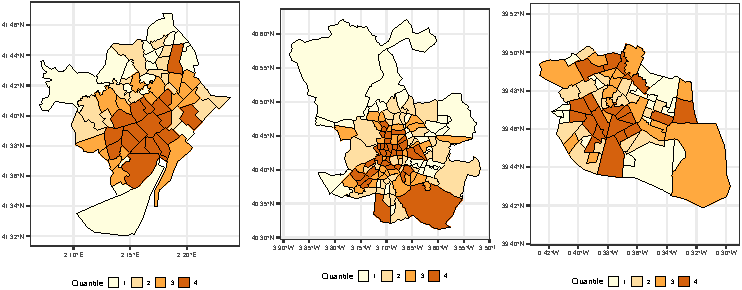
\includegraphics{EPB_files/figure-latex/unnamed-chunk-1-1.pdf}
\caption{\label{fig:all-polygons} (A) Weekly intra-province}
\end{figure}

There are a total of 73 neigborhoods in Barcelona, 135 in Madrid and 73
in Valencia. The sf object include an unique identifier (LOCATIONID) and
the neighborhood name (LOCATIONNAME).

\hypertarget{points-of-interest}{%
\subsection{Points of Interest}\label{points-of-interest}}

The last block of data included in the data package is a set of Point of
Interest of each city in \texttt{R} list R objetc. These lists include
three elements: (i) the coordinates of the city center (see that
identify the central business district); (ii) a set of points that
define the main street of each city; and (iii) the coordinates of metro
stations.

\hypertarget{sec:anonymizing}{%
\section{Anonymizing the data set}\label{sec:anonymizing}}

To comply with Spanish regulations, two variables are slightly modified
to preserve their anonymity. A masking process is apply to asking prices
and localization.

Whit respect to the asking prices, the original values are obfuscated
with the addition or subtraction of a random percentage of their
original values ranging from -2.5\% to +2.5\%. Since asking prices are
usually multiples of 1000, after the first price modification, the
prices was aligned to multiples of 1000.

With respect to the dwelling localization, a spatial masking process was
implemented with the intention of keeping spatial properties of the
original data set. The coordinates of each listing were displaced using
a stochastic procedure. Effectively, the listings were recorded using
coordinates contained in a maximum and minimum displacement circles, as
shown in Figure \ref{fig:points-moved-image}. To preserve membership in
a neighborhood, the spatial masking procedure was constrained to ensure
that the masked coordinates are in the original neighborhood of the
listing.

\begin{figure}[!ht]
  \caption{Masking coordinates. Spatial range}
  \centering
  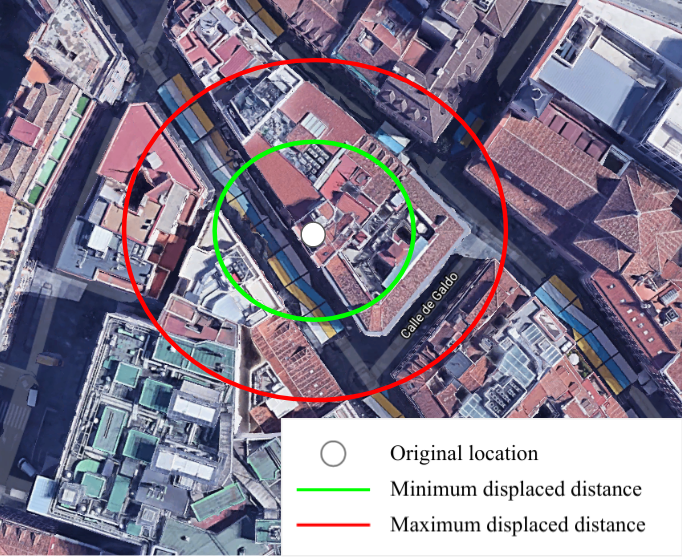
\includegraphics[width=6cm, height=4.9cm]{EPB_files/points-moved-image.png}
  \label{fig:points-moved-image}
\end{figure}

The algorithm \ref{algo:coordinates-displacement} iteratively displaces
the coordinates of each listing with a minimum distance and a maximum
distance with the restriction that the new coordinates do not fall in a
different neighborhood. This ensures that neighborhood attributes are
preserved.

\begin{algorithm}[!ht]
 \KwData{all idealista listings}
 \KwResult{all idealista listings with masked coordinates}
 initialization\;
 \For{each listing L}{
  take geographical location of L as $(X,Y)$
  \Repeat{this stop condition}{
    take a random angle $\alpha$ from 0 to 360 degrees
    take a distance $R$ as a random value from 30 to 60 meters
    determine a new point $(X',Y')$ calculated as a point located $R$ with the angle $\alpha$
  }
  set $(X',Y')$ as the new location for the listing L
 }
 \caption{Coordinate displacement process for anonymisation purposes}
 \label{algo:coordinates-displacement}
\end{algorithm}

Figure \ref{fig:coordinates-displacement} shows the histogram of
displacements in meters for all listings in the city of Valencia; the
average distance between the original and masked coordinates is 45
meters.

\begin{figure}[!ht]
  \caption{Masking coordinates. Spatial range}
  \centering
  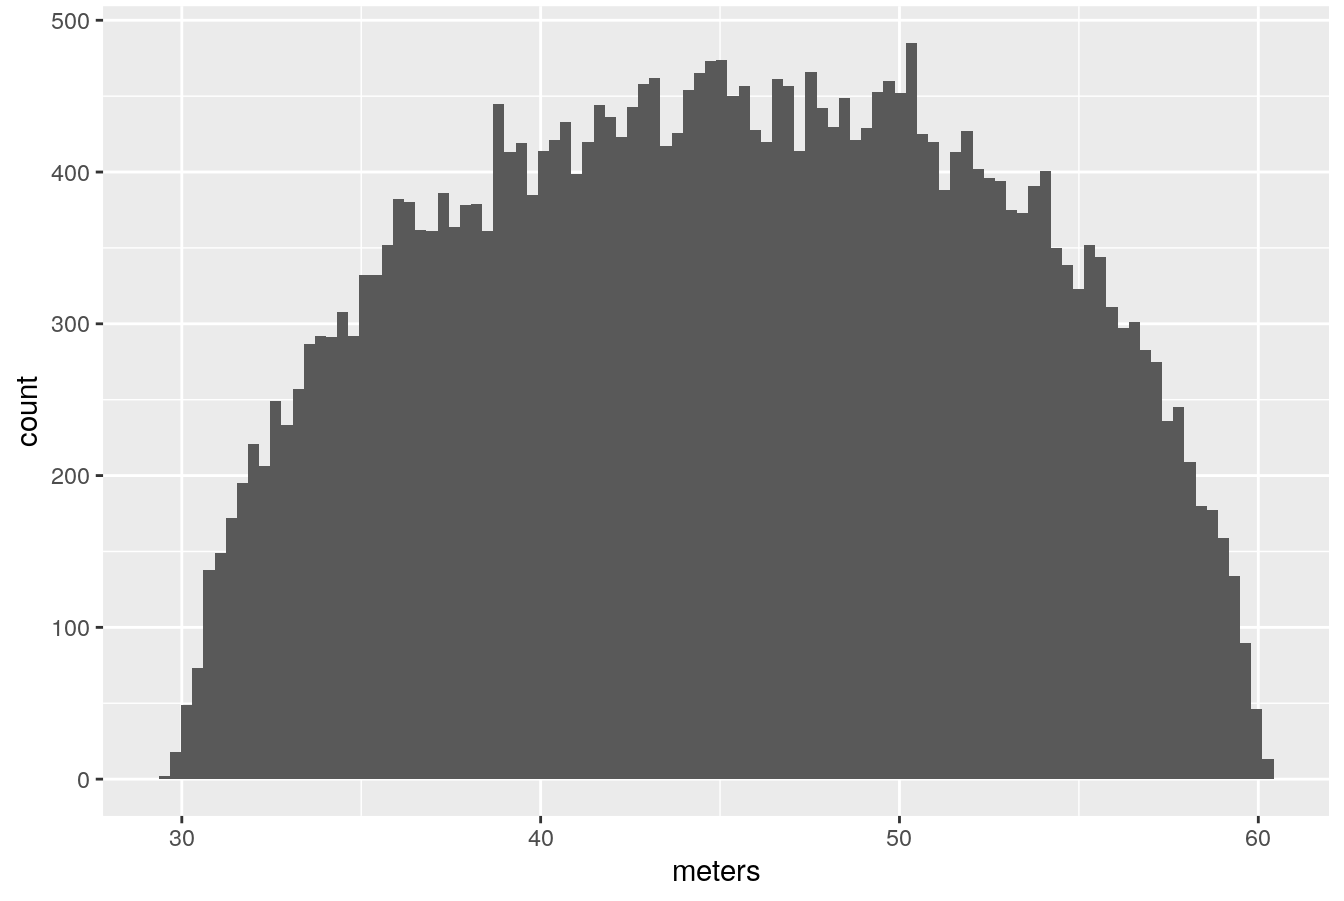
\includegraphics[width=6cm, height=4.9cm]{EPB_files/coordinates-valencia.png}
  \label{fig:points-moved-image}
\end{figure}

\hypertarget{the-geo-referenced-micro-data-set}{%
\subsection{The geo-referenced micro-data
set}\label{the-geo-referenced-micro-data-set}}

Spatial objects include geodetic coordinates using the \emph{EPSG:4326}
coordinate reference system.

\hypertarget{acknowledgments}{%
\section{Acknowledgments}\label{acknowledgments}}

The authors wish to thank Alessandro Galesi for their support in the
paper revision and Juan Ramon Selva for collecting and cleaning the
spatial data. This work has been partially funded by the Spanish
Ministry of Economy and Competitiveness Grants PID2019-107800GB- 100

\bibliographystyle{sageh}
\bibliography{bibEPB.bib}


\end{document}
